\section{离散型随机变量的概率分布}

\subsection{离散型随机变量的分布函数}

\begin{definition}[分布函数]
    设离散型随机变量 $ X $ 的分布律为
    $P\left\{X=x_{k}\right\}=p_{k},~k=1,2, \cdots,$ 则 $ X $ 的分布函数为
    $$F(x)=P\{X \leqslant x\}=\sum_{x_{k} \leqslant x} p_{k}$$
    或者
    $F(x)=\begin{cases}
            0,           & x<x_{1}                 \\
            p_{1},       & x_{1} \leqslant x<x_{2} \\
            p_{1}+p_{2}, & x_{2} \leqslant x<x_{3} \\
            \vdots       & \vdots
        \end{cases}$
\end{definition}

\begin{theorem}[分布函数的性质]
    以下三条是判定一个函数是否为分布函数的充要条件.
    \begin{enumerate}[label=(\arabic{*})]
        \item 单调性: $F(x) $ 是 $ x $ 的单调不减函数, 即对于任意实数 $ x_{1}<x_{2}$, 有 $ F\left(x_{1}\right) \leqslant F\left(x_{2}\right) $;
        \item 有界性: $\displaystyle0 \leqslant F(x) \leqslant 1 ,~F(-\infty)=\lim _{x \to-\infty} F(x)=0,~F(+\infty)=\lim_{x\to+\infty}F(x)=1$;
        \item 右连续: $F(x)$ 是 $x$ 的右连续函数, 即对任意实数 $x$, 有 $F(x^+)=F(x).$
    \end{enumerate}
\end{theorem}

\subsection{二项分布}

\begin{definition}[二项分布]
    在 $ n $ 重伯努利试验中, 若用随机变量 $ X $ 表示所关心事件 $ \sj{A} $ 发生的次数, $P(\sj{A})=p~~(0<p<1)$, 则 $ X $ 的分布律为
    $$P\{X=k\}=\C_{n}^{k} p^{k}(1-p)^{n-k}, ~k=0,1, \cdots, n$$
    则称 $ X $ 服从参数为 $ n, p $ 的二项分布, 记作 $ X \sim B(n, p) $.
    \begin{enumerate}[label=(\arabic{*})]
        \item 0-1 分布可以视为 $ n=1 $ 时的二项分布;
        \item 若 $ X \sim B(n, p) $, 令 $ Y=n-X$, 则 $ Y \sim B(n, 1-p) .$
    \end{enumerate}
\end{definition}

\subsection{泊松分布}

\begin{example}
    已知随机变量 $X_1 \perp  X_2$ 且分别服从参数为 $\lambda_1,~\lambda_2$ 的泊松分布, $P\qty{X_1+X_2>0}=1-\e ^{-1}$, 求 $E(X_1+X_2)^2$.
\end{example}
\begin{solution}
    $E(X_1+X_2)^2=EX_1^2+EX_2^2+2EX_1EX_2$, 且 $DX_i=EX_i^2-E^2X_i,~DX_i=EX_i=\lambda~(i=1,2)$, 故 
    $$
    E(X_1+X_2)^2=DX_1+E^2X_1+DX_2+E^2X_2+2EX_1EX_2=(\lambda_1+\lambda_2)+(\lambda_1+\lambda_2)^2
    $$
    而 $$
    P\qty{X_1+X_2>0}=1-P\qty{X_1+X_2\leqslant 0}=1-P\qty{X_1=0}P\qty{X_2=0}=1-\e ^{-(\lambda_1+\lambda_2)}
    $$
    于是 $\lambda_1+\lambda_2=1$, 故 $E(X_1+X_2)^2=1+1=2.$
\end{solution}

% \subsection{离散型随机变量的性质}
% 
% \begin{example}
%     设随机变量 $X$ 的概率分布 $P\qty{X=k}=\dfrac{a}{k(k+1)},k=1,2,\cdots,$, 其中 $a$ 为常数, $X$ 的分布函数为 $F(x)$, 已知 $F(b)=\dfrac{3}{4}$, 求 $b$ 的取值范围.
% \end{example}
% \begin{solution}
%     $\displaystyle \sum_{k=1}^{+\infty}P\qty{X=k}=\sum_{k=1}^{+\infty}\dfrac{a}{k(k+1)}=a\sum_{k=1}^{+\infty}\qty(\dfrac{1}{k}-\dfrac{1}{k+1})=a\lim_{k\to\infty}\qty(1-\dfrac{1}{k+1})=1\Rightarrow a=1$
%     则, $$F(x)=\sum_{k\leqslant x}\qty(\dfrac{1}{k}-\dfrac{1}{k+1})$$
%     当 $i\leqslant x<i+1$ 时, $$F(x)=\sum_{k\leqslant i}\qty(\dfrac{1}{k}-\dfrac{1}{k+1})=1-\dfrac{1}{i+1}$$
%     则 $F(b)=\dfrac{3}{4}=1-\dfrac{1}{4}\Rightarrow 3\leqslant b<4.$
% \end{solution}
% 
% \subsection{五大离散型分布}

\subsection{几何分布}

\begin{example}
    \begin{minipage}[t]{0.68\linewidth}
    飞行棋是一种家喻户晓的竞技游戏, 玩家根据骰子 (骰子为均匀的正六面体) 正面朝上的点数确定飞机往前走的步数, 刚好走到终点处算 “到达”, 如果玩家投掷的骰子点数超出到达终点所需的步数, 则飞机须往回走超出点数对应的步数, 在一次游戏中, 飞机距终点只剩 3 步 (如图所示), 设该玩家到达终点时投掷骰子的次数为 $X$, 则 $E(X)$ 等于 (\quad).
    \begin{tasks}(4)
        \task 2
        \task 4
        \task 6
        \task 8
    \end{tasks}
    \end{minipage}
    \begin{minipage}[t]{0.28\linewidth}
        \begin{figure}[H]
            \centering
            \tikzset{every picture/.style={line width=0.75pt}} %set default line width to 0.75pt        
            \begin{tikzpicture}[x=0.75pt,y=0.75pt,yscale=-1,xscale=1]
                %uncomment if require: \path (0,294); %set diagram left start at 0, and has height of 294
                
                %Up Arrow [id:dp6972322178564296] 
                \draw   (178,79.97) -- (198.33,60) -- (218.67,79.97) -- (208.5,79.97) -- (208.5,183.63) -- (188.17,183.63) -- (188.17,79.97) -- cycle ;
                %Shape: Ellipse [id:dp5499208028863829] 
                \draw   (188.79,76.7) .. controls (188.79,71.33) and (193.06,66.97) .. (198.33,66.97) .. controls (203.61,66.97) and (207.88,71.33) .. (207.88,76.7) .. controls (207.88,82.06) and (203.61,86.42) .. (198.33,86.42) .. controls (193.06,86.42) and (188.79,82.06) .. (188.79,76.7) -- cycle ;
                %Shape: Ellipse [id:dp015161662064077763] 
                \draw   (188.79,96.14) .. controls (188.79,90.77) and (193.06,86.42) .. (198.33,86.42) .. controls (203.61,86.42) and (207.88,90.77) .. (207.88,96.14) .. controls (207.88,101.51) and (203.61,105.86) .. (198.33,105.86) .. controls (193.06,105.86) and (188.79,101.51) .. (188.79,96.14) -- cycle ;
                %Shape: Ellipse [id:dp6960279033675896] 
                \draw   (188.79,115.58) .. controls (188.79,110.21) and (193.06,105.86) .. (198.33,105.86) .. controls (203.61,105.86) and (207.88,110.21) .. (207.88,115.58) .. controls (207.88,120.95) and (203.61,125.3) .. (198.33,125.3) .. controls (193.06,125.3) and (188.79,120.95) .. (188.79,115.58) -- cycle ;
                %Shape: Ellipse [id:dp057827204005403754] 
                \draw   (188.79,135.02) .. controls (188.79,129.65) and (193.06,125.3) .. (198.33,125.3) .. controls (203.61,125.3) and (207.88,129.65) .. (207.88,135.02) .. controls (207.88,140.39) and (203.61,144.74) .. (198.33,144.74) .. controls (193.06,144.74) and (188.79,140.39) .. (188.79,135.02) -- cycle ;
                %Shape: Ellipse [id:dp919946353596784] 
                \draw   (188.79,154.47) .. controls (188.79,149.1) and (193.06,144.74) .. (198.33,144.74) .. controls (203.61,144.74) and (207.88,149.1) .. (207.88,154.47) .. controls (207.88,159.83) and (203.61,164.19) .. (198.33,164.19) .. controls (193.06,164.19) and (188.79,159.83) .. (188.79,154.47) -- cycle ;
                %Shape: Ellipse [id:dp3503678725057724] 
                \draw   (188.79,173.91) .. controls (188.79,168.54) and (193.06,164.19) .. (198.33,164.19) .. controls (203.61,164.19) and (207.88,168.54) .. (207.88,173.91) .. controls (207.88,179.28) and (203.61,183.63) .. (198.33,183.63) .. controls (193.06,183.63) and (188.79,179.28) .. (188.79,173.91) -- cycle ;
                %Shape: Ellipse [id:dp3229416462640635] 
                \draw   (189.04,193.35) .. controls (189.04,187.98) and (193.31,183.63) .. (198.58,183.63) .. controls (203.85,183.63) and (208.13,187.98) .. (208.13,193.35) .. controls (208.13,198.72) and (203.85,203.07) .. (198.58,203.07) .. controls (193.31,203.07) and (189.04,198.72) .. (189.04,193.35) -- cycle ;
                %Image [id:dp5090881033363828] 
                \draw (198.13,135.07) node  {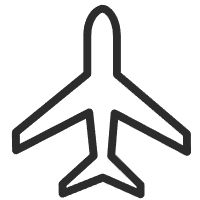
\includegraphics[width=14.32pt,height=14.58pt]{figures/aircraft.png}};
                
                
                % Text Node
                \draw (190.3,70) node [anchor=north west][inner sep=0.75pt]   [align=left] {{\tiny 终点}};
            \end{tikzpicture}
        \end{figure}
    \end{minipage}
\end{example}
\begin{solution}
    如图所示, 无论其具体位置如何, 一次投掷则可到达终点的概率始终为 $\dfrac{1}{6}$, 而有 $1-\dfrac{1}{6}=\dfrac{5}{6}$ 的概率转到下一轮投掷, 即 
    \begin{table}[H]
        \centering
        \begin{tabular}{c|cccccc}
            $X$ & 1 & 2 & 3 & $\cdots$ & $n$ & $\cdots$\\ 
            \hline
            $P$ & $\dfrac{1}{6}$ & $\dfrac{5}{6}\times\dfrac{1}{6}$ & $\qty(\dfrac{5}{6})^2\times\dfrac{1}{6}$ & $\cdots$ & $\qty(\dfrac{5}{6})^{n-1}\times\dfrac{1}{6}$ & $\cdots$ 
        \end{tabular}
    \end{table}
    即 $X$ 服从参数为 $p=\dfrac{1}{6}$ 的几何分布, $E(X)=\dfrac{1}{p}=6.$
\end{solution}